\documentclass[12pt]{article}

%!TEX root = main.tex

% for subfigures
\usepackage[textfont={it,scriptsize}]{subfig}

\usepackage[vlined, boxed,linesnumbered,noend]{algorithm2e}

\usepackage{cprotect}
\usepackage{booktabs}
\let\proof\relax
\let\endproof\relax
\usepackage{amsthm}
\usepackage{amsmath,amssymb,mathtools,stmaryrd}
%\usepackage{latexsym}
\usepackage{graphicx}
\usepackage{complexity}
\usepackage{tikz}
\usepackage{xspace}
%\usepackage{verbatim}
\usepackage{multicol}
%\usepackage{fancybox}
\usepackage{wrapfig}
\usepackage{enumitem}
%\usepackage{paralist}
\usepackage[bottom]{footmisc}
\usepackage{footnote}
\makesavenoteenv{table}
\makesavenoteenv{tabular}
%\usepackage{pbox}
%\usepackage{float}
\usepackage[font={scriptsize,it}]{caption}
%\usepackage[font={scriptsize,it}]{subcaption}
\usepackage{adjustbox}
\usepackage{color}
% For striking out text:
\usepackage{cancel}
\usepackage[normalem]{ulem}
%\usepackage[nounderscore]{syntax}


% For Arxiv:
\usepackage{ifpdf}
    \ifpdf
\usepackage[colorlinks,citecolor=blue!60!black!70,linkcolor=blue!60!black!70]{hyperref}
    \else
%      do something for regular latex or pdflatex in dvi mode
    \fi


\usetikzlibrary{automata}
\usetikzlibrary{positioning}
%\usetikzlibrary{decorations.pathmorphing}
\usetikzlibrary{arrows,patterns}
\usetikzlibrary{calc}
\usetikzlibrary{decorations.pathreplacing,decorations.markings}


\renewcommand\paragraph[1]{\vspace{.0ex}\par\noindent\textbf{#1}.\;\;}
\newtheorem{observation}{Observation}
\newtheorem{alg}{Algorithm}

\renewcommand{\topfraction}{0.9}
\renewcommand{\bottomfraction}{0.9}


\def\sectionautorefname{Sec.}
\def\subsectionautorefname{Sec.}
\def\corollaryautorefname{Cor.}
\def\definitionautorefname{Def.}
\def\figureautorefname{Fig.}
\def\exampleautorefname{Ex.}
\def\algorithmautorefname{Alg.}
\def\appendixautorefname{App.}
\def\algautorefname{Alg.}
\def\observationautorefname{Obs.}
\def\lemmaautorefname{Lemma}
\def\theoremautorefname{Th.}
\def\equationautorefname{Eq.}
\newcommand{\subfigureautorefname}{\figureautorefname}


\let\ssaphi=\phi % Georg: I need the original phi
\let\phi=\varphi 
\let\epsilon=\varepsilon
\let\code=\verb
\renewcommand\implies{\Rightarrow}


\hyphenation{bet-ween}
\hyphenation{da-ta-base}
\hyphenation{wor-ker}



%%% Local Variables: 
%%% mode: latex
%%% TeX-master: "main"
%%% End: 

%!TEX root = main.tex


\newcommand\defaccr[2]{\newcommand#1{#2\xspace}}
\newcommand\defmath[2]{\newcommand#1{\ensuremath{#2}\xspace}}
\newcommand\concept[1]{\textit{#1}}



\newcommand\ccode[1]{\texttt{#1}}


\newcommand{\overarrowi}[1]{\xrightarrow{#1}}
\newcommand{\overarrow}[1]{
  \mathchoice{\raisebox{-3pt}{ $\overarrowi{#1}$ }}
             {\raisebox{-3pt}{ $\overarrowi{#1}$ }}
             {\raisebox{-3pt}{ $\overarrowi{#1}$ }}
             {\raisebox{-3pt}{ $\overarrowi{#1}$ }}}

%containers
\providecommand{\tuple}[1]{\ensuremath{\left( #1 \right)}}
\providecommand{\set}[1]{\ensuremath{\left\lbrace #1 \right\rbrace}}
\providecommand{\sequence}[1]{\ensuremath{\left( #1 \right)}}
\providecommand{\sizeof}[1]{\ensuremath{\left\vert{#1}\right\vert}}
\providecommand{\vect}[1]{\ensuremath{( \begin{matrix} #1 \end{matrix} )}}
\providecommand{\always}[1]{\ensuremath{\left[ #1 \right]}}
\providecommand{\possibly}[1]{\ensuremath{\left\langle #1 \right\rangle}}
%\newcommand{\powerset}[1]{\wp({#1})}
\newcommand{\powerset}[1]{\ensuremath{\mathbf{2}^{#1}}}
% Semantics
\newcommand{\eval}[2][]{\ensuremath{\llbracket #2\rrbracket^{#1}}}

% Map (bijection)
\DeclareMathOperator{\bijmap}{%
 \rlap{\ensuremath{\rightarrowtail}}%
 	{\ensuremath{\mkern2mu\twoheadrightarrow}}}

% Abs, Floor, Ceil
\providecommand{\abs}[1]{\lvert#1\rvert}
\providecommand{\floor}[1]{\lfloor#1\rfloor}
\providecommand{\ceil}[1]{\lceil#1\rceil}

\newcommand{\defn}{\,\triangleq\,}

% Rotate text
\newcommand{\turner}[3][10em]{% \turn[<width>]{<angle>}{<stuff>}
  \rlap{\rotatebox{#2}{\begin{varwidth}[t]{#1}#3\end{varwidth}}}%
}


\providecommand{\Assign}[2]{{#1{~:=~}#2}}
\providecommand{\AssignState}[2]{\State \Assign{#1}{#2}}


%initial state
\newcommand{\inits}{s^0}

%transition relation expression
\newcommand{\transrelexpr}{\mathsf{next}}%\mathord{\hookrightarrow}}

\defmath{\explored}{\mathsf{explored}}
\defmath{\visited}{\mathsf{visited}}
\defmath{\level}{\mathsf{level}}
\defmath{\tmp}{\mathsf{tmp}}
\defmath{\WM}{\mathsf{WM}}
\defmath{\RM}{\mathsf{RM}}
%next state small caps
\renewcommand{\next}{\mathsf{next}}

%next state small caps
\newcommand{\nextstate}{\textsc{next-state-r2w}\xspace}

%!TEX root = main.tex


\defmath\dna{\ensuremath\mathcal{\not\bowtie}}
\defmath\B{\ensuremath\mathit{B}}

\newcommand\en{\ensuremath{\mathit{en}}\xspace}
\newcommand\modell{\ensuremath{M_{\structuraltransitions}}\xspace}
\newcommand\modelr{\ensuremath{\modell^R}\xspace}
\newcommand\buchi{\ensuremath{\mathbb{B}}\xspace}
\newcommand\accepting{\ensuremath{\mathcal{F}}\xspace}
\newcommand\cross{\ensuremath{\modell\otimes \buchi_{\neg\varphi}}\xspace}
\newcommand\crossr{\ensuremath{\modell^R\otimes \buchi_{\neg\varphi}}\xspace}

\newcommand\vis{\ensuremath{\structuraltransitions_\mathrm{v}}\xspace}
\newcommand\vismax{\ensuremath{\vis^\mathrm{min}}\xspace}
\newcommand\vislabels{\ensuremath{\vis^\mathrm{nes}}\xspace}
\newcommand\visdyn{\ensuremath{\vis^\mathrm{dyn}}\xspace}

\renewcommand\implies{\Rightarrow}

\newcommand{\instantiator}{\textsc{Instantiator}\xspace}
\newcommand\nips{\tool{Nips}}
\newcommand\nipsvm{\nips\-\tool{VM}\xspace}
\newcommand\spin{{\sc Spin}\xspace}
\newcommand\spinja{{\sc SpinJa}\xspace}
\newcommand\promela{\textsc{Promela}\xspace}
\newcommand\dve{\textsc{Dve}\xspace}
\newcommand\beem{\textsc{BEEM}\xspace}
\newcommand\divine{\tool{DiVinE}\xspace}
\newcommand\mcrl{\ensuremath{\mu\mathrm{CRL}}\xspace}
\newcommand\mcrltwo{mCRL2\xspace}
%\newcommand\pins{\iface{Pins}\xspace}
\newcommand\pinspins{\iface{Pins2Pins}\xspace}
\newcommand\cadp{CADP\xspace}
\newcommand\ltsmin{{\sc LTSmin}\xspace}

\newcommand{\statevec}[1]{\ensuremath{\langle{#1}\rangle_{\mathrm{SV}}}}
\newcommand{\intvec}[1]{\ensuremath{\langle{#1}\rangle_{\mathrm{IV}}}}
\newcommand{\foldedvec}[1]{\ensuremath{\langle{#1}\rangle_{\mathrm{FV}}}}
\newcommand{\pair}[1]{\ensuremath{\langle{#1}\rangle}}

\newcommand{\Nat}{\ensuremath{\Bbb N}}
\newcommand{\Bool}{\ensuremath{\Bbb B}}
\DeclareMathOperator{\hash}{Hash}
\newcommand{\statepart}[1][s]{#1}

\newcommand{\struct}[1]{\ensuremath{\langle#1\rangle}}

\newcommand\logor{\vee}
\newcommand\logand{\wedge}
\newcommand{\var}[1]{\ensuremath\mathit{#1}}

\newcommand\true{\ensuremath\textbf{true}}
\newcommand\false{\ensuremath\textbf{false}}
\newcommand\guards{\ensuremath\mathcal{G}}
\newcommand\allguards{\ensuremath{\guards_{\structuraltransitions}}}
\newcommand\initialstate{\ensuremath{s_0}}
\newcommand\structuraltransitions{\ensuremath\mathcal T}
\newcommand\semantictransitions{\ensuremath\Delta}
\newcommand\states{\ensuremath{S}}
\newcommand\modelstates{\ensuremath {S_{\structuraltransitions}}}
\newcommand\model{\ensuremath{M_{\structuraltransitions} = (\modelstates,\initialstate,\semantictransitions)}}
\newcommand\structuraltransition{\ensuremath{t = (\guards,a)}}
\newcommand\stateelements{\ensuremath{E_1 \times \ldots \times E_n}}
\newcommand\testset{\ensuremath{\mathit{Ts}}\xspace}
%\newcommand\readset{\ensuremath{\mathit{Rs}}\xspace}
%\newcommand\writeset{\ensuremath{\mathit{Ws}}\xspace}
\newcommand\variableset{\ensuremath{\mathit{Vs}}\xspace}
\newcommand\MC{\ensuremath{\mathit{MC}}\xspace}
\newcommand\findnes{\ensuremath{\mathit{find\_nes}}\xspace}
\newcommand\persistentset{\ensuremath{\mathcal{T}}\xspace}
\newcommand\stubbornset{\ensuremath{\mathcal{T}_s}\xspace}
\newcommand\workset{\ensuremath{Q}\xspace}
\newcommand\keyset{\ensuremath{\mathcal{T}_{\mathit{k}}}\xspace}
\newcommand\nkset{\ensuremath{\mathcal{T}_{\mathit{n}}}\xspace}
%\newcommand\nes{\ensuremath{\mathcal{N}}\xspace}
\newcommand\nesmax{\ensuremath{\nes^\mathrm{min}}\xspace}
\newcommand\nespins{\ensuremath{\nes^\textsc{pins}}\xspace}
\newcommand\nds{\ensuremath{\overline{\nes}}\xspace}
\newcommand\mds{\ensuremath{\mathcal{M}}\xspace}
\newcommand\ndsmax{\ensuremath{\nds^\mathrm{min}}}
\newcommand\ndspins{\ensuremath{\nds^\textsc{pins}}}

\newcommand\trans\structuraltransitions
\newcommand\transitions\structuraltransitions


%%% Local Variables: 
%%% mode: latex
%%% TeX-master: "main"
%%% End: 


\title{Partial Order Reduction}

\author{{Alfons Laarman, Pim Wijn}}


\pagestyle{plain}

\def\ltsmin{\textsc{LTSmin}\xspace}


\begin{document}




\maketitle

\section{Introduction}

The current lab assignment lets you implement a basic
partial order reduction algorithm. 
The next-state interface is again used for
on-the-fly model checking. 
This time the model checker \texttt{mc.cpp}
is slightly extended to make use of a slightly more
extended version of the next-state interface, called
Partitioned Next-State Interface (PINS).

Apart from a next-state function, PINS also exposes
static information about the model.
A read and write boolean matrix $R_{i,j}$/$W_{i,j}$
provides an overestimation
of which variables $j$ in the state vector are read / 
written to by which action $i$ (or group in PINS terminology).
Furthermore, a state label matrix $L_{i,j}$ contains information
about which variables $j$ in the state vector are read
when evaluating a state label $i$.
Other matrices exposes the non-commutativity information
(actions $\times$ actions), the action to guard relation 
(action $\times$ state labels) and 
necessary enabling information (labels $\times$ actions).
We will use this information to implement POR.
More details follow, but the full PINS interface is described in~\cite{ltsmin2}.


Extract the zip file from blackboard and make 
sure \ltsmin is still installed.\footnote{In Lab 1,
\ltsmin was installed in \texttt{\$HOME/ltsmin}.
Make sure \texttt{\$HOME/ltsmin/bin} is still in your
\texttt{\$PATH}, i.e., the commands \texttt{pins2lts-mc} and \texttt{spins} are executable.}
The code can be compiled with the following commands:

\texttt{cmake .}

\texttt{make}


To run the model checker call:

\texttt{./mc <model>}

Here, \texttt{<model>} can be a Promela model
from the examples dir (which should be compiled
automatically to a \texttt{.spins} library
provided that \texttt{spins} is in your path).
Alternatively, the Peterson from Lab 1 model can 
still be used. It is compiled to \texttt{libpeterson.so}
in the \texttt{peterson} subdir. It can thus be run with:

\texttt{./mc peterson/libpeterson.so}


\section{Introduction to Callback Functions}

To implement iterators, PINS uses callback functions.
Passing these callbacks is based on function pointers.
Function pointers are literally pointers to
\emph{function implementations}.
They can be used to parametrize the called function:
\begin{verbatim}
typedef int (*function_pointer_type)(int a, int b);
int function_implementation(int a, int b) { return a * b; }
int main(){
    function_pointer_type fp = function_implementation;
    assert (fp(4,99) == function_implementation(4,99));
}
\end{verbatim}
PINS passes function pointers to implement iteration efficiently.
In a simple world, the \texttt{GBgetTransitionsAll} function
could return a set of successors to iterate on, as follows:
\begin{verbatim}
void search(stack_t *stack) {
    ...
        for (int *dst : GBgetTransitionsAll(model, src)) {
            stack_push(stack, dst);
        }
    ...
}
\end{verbatim}
To avoid creating this set storing all
the vectors, instead we do the following:
\begin{verbatim}
static stack_t *stack;

void callback(void *context, transition_info_t *ti, int *dst, int *cpy) {
    stack_push(stack, dst);
}
void search() {
    ...
        GBgetTransitionsAll(model, src, callback));
    ...
}
\end{verbatim}
Notice that we can no longer use local variables in the callback
and hence, we had to declare stack a static global variable.
To avoid this, callbacks additionally take a pointer to a
``context''. With some casting, we can now pass around the variables we need:
\begin{verbatim}
void callback(void *context, transition_info_t *ti, int *dst, int *cpy) {
	stack_t *stack = (stack_t *) context;
    stack_push(stack, dst);
}
void search(stack_t *stack) {
    ...
        GBgetTransitionsAll(model, src, callback, (void *) stack));
    ...
}
\end{verbatim}



\section{Partial Order Reduction}

Partial order reduction (POR) will be implemented 
in an extra layer in the next-state interface, which
intercepts next-state calls to model, computes an
ample set and only passes those actions through to 
the callee (the state space search algorithm) that are in the ample set.

\defmath\nes{nes}
\begin{center}
\newcommand\alert[1]{{\color{orange}#1}}
\defmath\pins{\textsc{pins}}
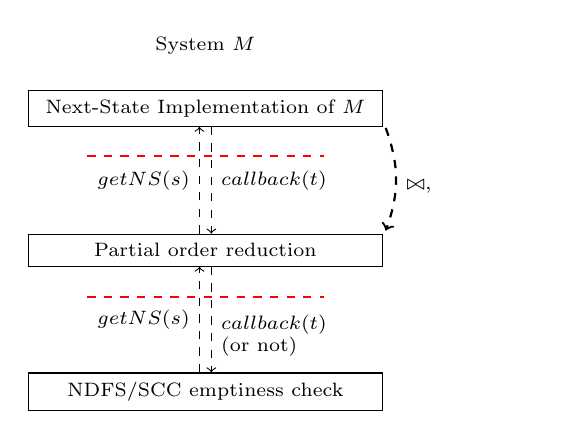
\begin{tikzpicture}[font=\scriptsize]
\tikzstyle{every node}=[draw,shape=rectangle,node distance=1.8cm];
\node (a0) [minimum  width=4.5cm] {NDFS/SCC emptiness check};
%\node (a1) [above of=a0, minimum  width=4.5cm] {LTL crossproduct $M\otimes \mathcal B_\varphi$};

{
\node (a2) [above of=a0,minimum  width=4.5cm] {Partial order reduction};
}

\node (a3) [above of=a2,minimum  width=4.5cm] {Next-State Implementation of $M$};
\node (spec) [above of=a3,draw=none,node distance=.8cm,minimum  width=4.5cm]
{System $M$};
%\node (prop2) [right of=spec,draw=none,node distance=4cm]{\phantom{Property $\varphi$}};
%\node (prop) [left of=spec,draw=none,node distance=4cm]{Property $\varphi$};


{
%\draw[transform canvas={xshift=-.5ex},->,dashed] (a1) -- node[left,draw=none]{$getNS(s)$}(a3);
%\draw[transform canvas={xshift=.5ex},->,dashed] (a3) -- node[right,draw=none]{$callback(t)$}(a1);
}
{
%\draw[transform canvas={xshift=-.5ex},->,dashed] (a1) -- node[left,draw=none]{$getNS(s)$}(a2);
\draw[transform canvas={xshift=.5ex},->,dashed] (a2) -- node[yshift=-.2cm,text width=1.5cm,right,draw=none]{$callback(t)$ \alert{(or not)}}(a0);
\draw[transform canvas={xshift=-.5ex},->,dashed] (a2) -- node[left,draw=none]{$getNS(s)$}(a3);
\draw[transform canvas={xshift=.5ex},->,dashed] (a3) -- node[right,draw=none]{$callback(t)$}(a2);
}
\draw[transform canvas={xshift=-.5ex},->,dashed] (a0) -- node[left,draw=none]{$getNS(s)$}(a2);
%\draw[transform canvas={xshift=.5ex},->,dashed] (a1) -- node[right,draw=none]{$callback(t')$}(a0);\draw[->,thick] (spec) -- (a3);
%\draw[->,thick] (prop) -- (a3);

\tikzstyle{every node}=[node distance=1.1cm,scale=2];
\node (b0) [right of=a0,draw=none] {};
%\node (b1) [right of=a1,draw=none] {};
%\node (bb1) [right of=b1,xshift=.1cm,draw=none] {};
\node (b2) [right of=a2,draw=none] {};
\node (b3) [right of=a3,draw=none] {};

%\draw[->,thick] (prop) edge[bend right=25] (a1.west);

\tikzstyle{every node}=[node distance=2cm]


{
\draw[->,dashed,thick] (b3) edge [bend left=20] node[text width=1.5cm,yshift=-.1cm,right]{$\bowtie, \nes$} (b2);
}{
%\draw[->,dashed,thick] (a1.east) edge [bend right=25] node[yshift=-.15cm,left]{$\underline{Vis}$} (a2.east);
}

{
%\draw[->,dashed,thick] (b0) edge [bend right=60]
%node[xshift=-.3cm,yshift=-.9cm,text centered,text width=2.5cm,right]
%{\underline{$s\in \mathit{stack}$}
%($s$~lies~on~a~cycle) } (b2);
}

%\draw[-,dashed,thick,color=red] (-1.5,4.8) -- node[xshift=-1.9cm,yshift=-0em]{\pins} (1.5,4.8);

{
\draw[-,dashed,thick,color=red] (-1.5,3) -- node[xshift=-1.9cm,yshift=-0em]{\pins} (1.5,3);
}
\draw[-,dashed,thick,color=red] (-1.5,1.2) -- node[xshift=-1.9cm,yshift=-0em]{\pins} (1.5,1.2);
\end{tikzpicture}
\end{center}


The POR layer is implemented in \texttt{por/por.c}.
It is activated by calling \texttt{./mc} with an
additional \texttt{--por} argument.
The initial implementation of \texttt{por.c}
does nothing but forward the incoming next-state calls,
i.e., to return all successors of the \texttt{src} state,
so no reduction results from activating the layer.


\begin{algorithm}[b]
\SetKwBlock{Function}{function}{end function}
\Function({$\mathit{stubborn}_{\mathit{closure}}(s)$}) {
$\workset = \{{\alpha} \}$ \textbf{for some} ${\alpha} \in \en(s)$\\\label{l:nondet1}
$\stubbornset = \emptyset$\\
\While{$\workset \neq \emptyset$}{
    $\workset = \workset \setminus \{\alpha\}$,
    $\stubbornset = \stubbornset \cup \{\alpha\}$ \textbf{for some} $\alpha \in \workset$\\
    \eIf{$\alpha \in \en(s)$}{
        $\workset = \workset \cup \dna(\alpha) \setminus \stubbornset$\\\label{closure:en}
    }
    {
        $\workset = \workset \cup \nes(g) \setminus  \stubbornset$ \textbf{for some}
        guard $g \in G(\alpha)$ \textbf{s.t.}
        $\neg g(s)$\\\label{l:nondet2}
    }
}
\Return{$\stubbornset \cap \en(s)$}
}
\caption{The \concept{closure} algorithm for finding stubborn sets}
\label{alg:stubborn-set}
\end{algorithm}


The task is to implement the stubborn set in order
to find a sufficient subset of actions enabled from
\texttt{src}, to reduce the state space while
retaining all of its its deadlocks.
The POR algorithm is also a search, but over the
actions, enabled and disabled in the source state.
The \texttt{por\_next\_all} function contains some hints about
how this search over actions that can be implemented.

\autoref{alg:stubborn-set} describes a
 simple algorithm to compute a stubborn set \stubbornset for a state~$s$.
The visited actions are recorded in the stubborn set \stubbornset and
new actions are added to the queue \workset (\texttt{por->actions\_selected} and
\texttt{por->queued} in the code).


The algorithm further relies on actions $\alpha$ having a set of guards (state labels)
that can be evaluated in the state. A guard $g\in G(\alpha)$ of $\alpha$ is
disabled in $s$ when $\neg g(s)$ and enabled in $s$ when $g(s)$
(\texttt{GBgetGuard()} in the code implements $G$ and 
\texttt{por->guard\_status[g]} implements $g(s)$/$\neg g(s)$).

The non-commuting actions for an actions $\alpha$ are
denoted with $\not\bowtie\hspace{-1.5mm}(\alpha)$ (\texttt{por->ncommute} in the code).
For enabled actions in the stubborn set \stubbornset, all non-commuting
actions should be added (see Line 7).
For a  disabled action $\alpha$ in the stubborn set,
a complete necessary enabling set (\texttt{por->nes} in the code)
should be added for at least one disabled guard of $\alpha$ (see Line 9).


The \texttt{X.509} protocol in the \texttt{examples} dir has 9028 states and
4 deadlocks. Does your reduction implementation retain all deadlocks?
How many states does the reduced state space contain?
How well do other models reduce?

\texttt{./mc X.509.pr.spins --por}

 
Improvements to this basic algorithm and also a more advanced algorithm, can be
found in \cite{guardpor2}.

\begin{proof}[Bonus assignment 1]
	To use the reduction on your Peterson model, copy your version of
	\texttt{peterson.c} in the peterson dir and extend 
	\texttt{peterson.c} and \texttt{dlopen-impl.c} to pass
	the required to information to the PINS interface:
	\texttt{GBsetNextStateLong} (for evaluating state labels),
	\texttt{GBsetStateLabelInfo} (for indicating which state slots are read by the guards),
	\texttt{GBsetGuardsInfo} (for $G$, i.e., assigning guards to actions (groups)),
	\texttt{GBsetGuardNESInfo} (for the NES matrix), and
	\texttt{GBsetDoNotAccordInfo} (for the non-commute matrix).
	The latter two can be estimated from the state slots read/written 
	by actions and guards (see the included \texttt{peterson.c} for an example).
\end{proof}

\begin{proof}[Bonus assignment 2]
Improve the performance and memory usage of the model checker further by using
the tree compression data structure. An implementation of the structure 
can be found in \texttt{util-mc/treedbs-ll.c}.
\end{proof}



\section{Hand in Results}

Write a short report (as short as possible) answering the above questions and zip it together with
your source code.
Hand in your results in the `Labs' section on Blackboard.



\bibliographystyle{plain}
\bibliography{lit}


\end{document}

%%% Local Variables:
%%% mode: latex
%%% TeX-master: t
%%% End:
